\clearpage{\pagestyle{empty}\cleardoublepage}

\chapter{Theoretical framework}\label{chap:TH}

\vspace{-2.5cm}

%\epigraph{Today I have done something which no theoretical physicist should ever do in his life: I have predicted something which shall never be detected experimentally!}{Wolfang Pauli to his friend Walter Baade}
\begin{flushright}
\begin{minipage}{.6\textwidth}
\begin{flushright}

\vskip5pt

\hrule 

\vskip7pt

{\it Today I have done something which no theoretical physicist should ever do in his life: I have predicted something which shall never be detected experimentally!}

\vskip5pt

\small{Wolfang Pauli to his friend Walter Baade}

\hrule

\vskip5pt


\end{flushright}
\end{minipage}
\end{flushright}


\vspace{0.5cm}

The Standard Model of particle physics is a
successful, mathematically-elegant and precise 
theory describing the interactions
between fundamental particles. 
Over the last few decades it has been verified experimentally
up to a very high degree of accuracy, most notably by precision measurements 
%Its validity has been tested by precision measurements 
at the Large Electron-Positron Collider at CERN.
The Standard Model has been further confirmed 
by the observation of all the particles it 
predicts, including the Higgs-like boson discovered at the
Large Hadron Collider in July of 2012 which up to now 
behaves as expected from this theory.

However, unstabilities appear at high energy scales 
of the order of the Planck mass in the mathematical formulation.
This makes the Standard Model more like an {\it effective theory}, 
valid up to a certain energy scale, than a complete and final framework.
In this chapter we will first overview in Section~\ref{sec:THsm} the milestones
in the history of particle physics that lead to the construction
of the Standard Model, presented in Section~\ref{sec:THlagr}.
Section~\ref{sec:THquest} is dedicated to the
open questions that hint at the Standard Model 
as an effective theory and whose solutions are proposed
in the ``New Physics'' models like the ones described.
Some of them predict the presence of new heavy and exotic
quarks, namely {\it vector-like quarks}, which are
the objects hunted by the analyses presented in this dissertation.
A brief description of their properties and phenomenology is
given in Section~\ref{sec:THvlq}.


\section{The road to the Standard Model: particle physics from 1936 to 2012}\label{sec:THsm}

During the first half of the 20th century, many experimental 
discoveries were challenging particle physicists to find a 
coherent model to explain the existence of new particles and 
forces. A ``heavy electron'', the muon, was observed in 1936 
by C. %arl 
 Anderson and S. %eth 
 Neddermeyer in cosmic radiation, and later
observed in a cloud chamber experiment by %Jabez Curry 
J. C. Street and E. C. Stevenson~\cite{PhysRev.52.1003}. 
The neutrino, postulated in 1930 by %Wolfgang
W. Pauli\footnote{Pauli did not write a scientific
paper of his great intuition, which is only testified 
by a letter he sent to the 1930 Gauverein meeting in T\"ubingen,
famous also for his funny opening 
``{\it Dear Radioactive Ladies and Gentlemen,[\dots]}''. A copy
of the letter can be found in \url{http://tinyurl.com/cjgoubj}, 
and a nice overview on the history of the neutrino is in~\cite{2006physics...3106P}.}
to explain the shape of the electron 
spectrum in beta decay, was experimentally 
detected in 1956 by %Clyde L. 
C. L. Cowan and %Frederick 
F. Reines~\cite{1956Sci...124..103C}, and few years later a 
second neutrino type was discovered by %Leon M. 
L. M. Lederman, %Melvin 
M. Schwartz and %Jack 
J. Steinberger~\cite{1962PhRvL...9...36D}. 
By 1963 a huge number of new {\it mesons} and {\it baryons} 
were populating what was called the ``particle zoo'' 
until Murray Gell-Mann and George Zweig independently proposed 
a classification for all these new particles 
supposing that hadrons were made by three smaller 
components named {\it quarks}~\cite{GellMann1964214,Zweig:352337}
and dotated of a new
quantum number, the hypercharge $Y=2(Q-I_3)$, where $Q$ is the electric
charge and $I_3$ the third componend of the isospin.
Figure~\ref{fig:eightfold} shows this particle classification referred to as 
``the eightfold way''\footnote{See e.g. \url{http://lccn.loc.gov/65013009}.}. 

\begin{figure}[h!tb]\begin{center}
	\subfigure[]{
  	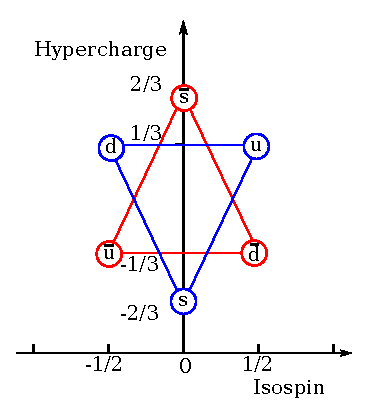
\includegraphics[width=0.3\textwidth]{theory/figures/threequarks}}\\
	\subfigure[]{
  	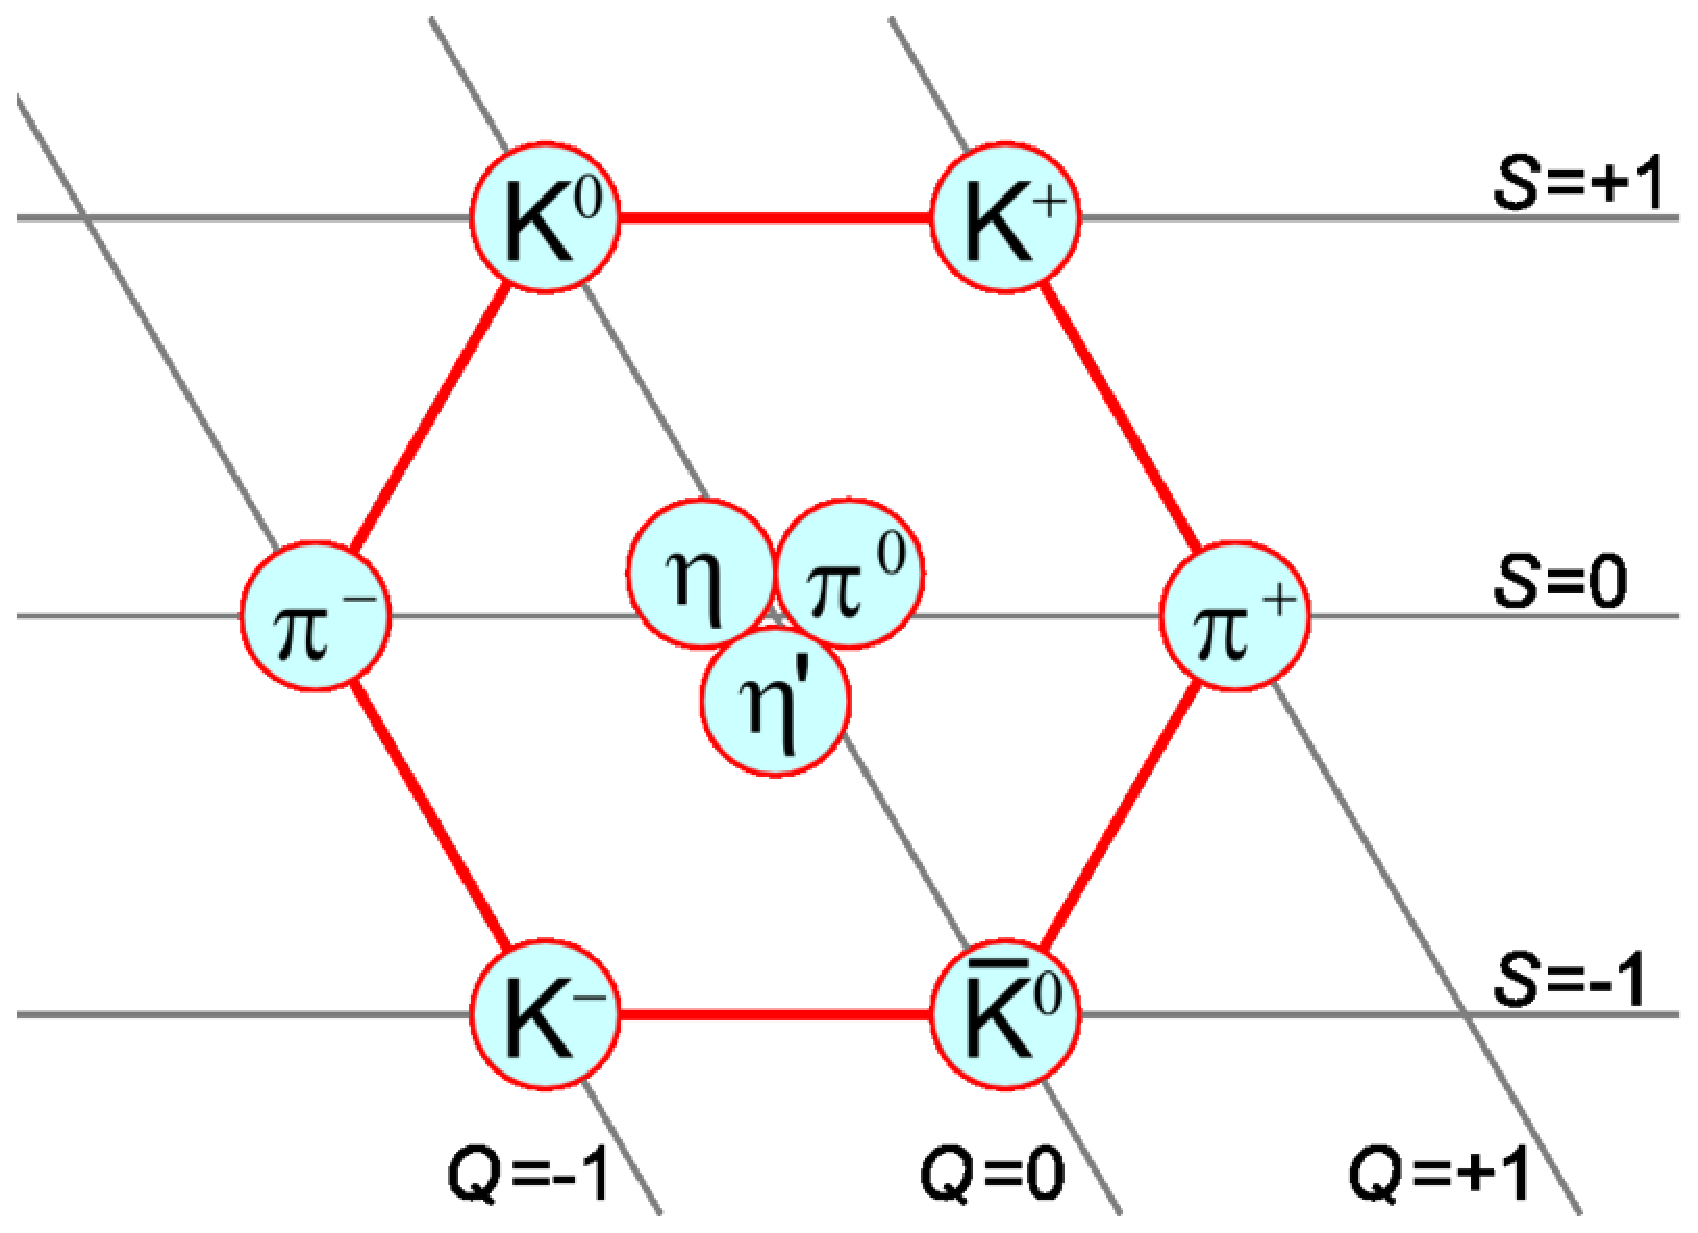
\includegraphics[width=0.37\textwidth]{theory/figures/mesons}}
	\subfigure[]{
  	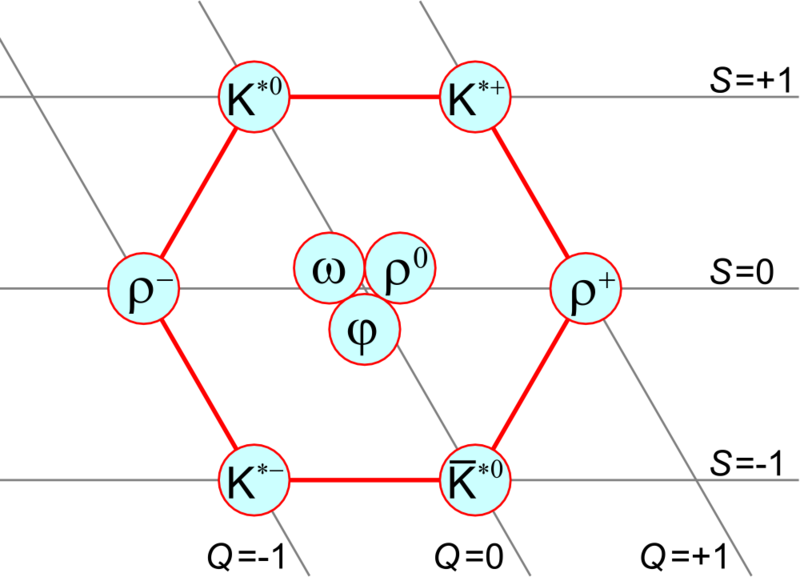
\includegraphics[width=0.37\textwidth]{theory/figures/mesons1}}
	\subfigure[]{
  	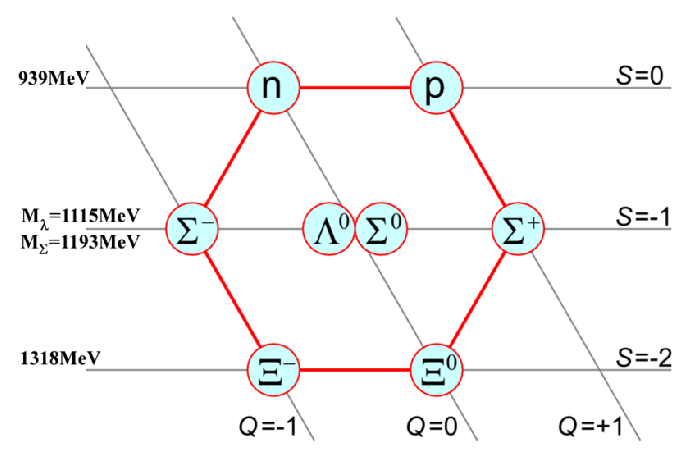
\includegraphics[width=0.4\textwidth]{theory/figures/Baryon_octet_w_mass}}
	\subfigure[]{
 	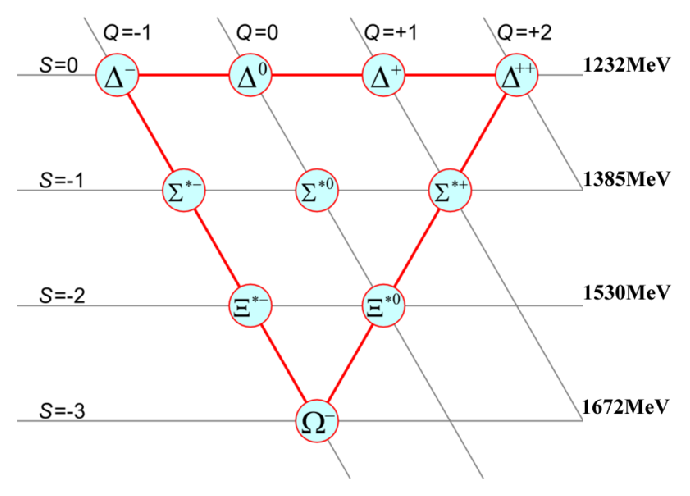
\includegraphics[width=0.4\textwidth]{theory/figures/Baryon_decuplet_w_mass}}
	\caption{Gell-Mann's \textit{Eightfold Way} (proposed also independently 
          by Yuval Ne'eman) identifies three fundamental components (a) 
          and classifies through their electric charge $q$ and strangeness $s$:
          a spin-0 meson octet (b), a spin-1 meson octet (c), 
          a spin-1/2 baryon octet (d) and a spin-3/2 baryon decuplet (e).
          It is now understood that this structure is a 
          consequence of a flavour symmetry.\label{fig:eightfold}}
\end{center}\end{figure}

It was the beginning of the {\it quark model}, a theory that had to 
wait for multiple experimental evidence before being accepted,
nevertheless it successfully predicted a new particle, the strangeness $s$=-3 
particle $\Omega^{-}$ of the spin-3/2 baryon decuplet of Figure~\ref{fig:eightfold},
discovered in 1964 at Brookhaven~\cite{PhysRevLett.12.204}. 
Even when in 1968 deep inelastic experiments at the Stanford 
Linear Accelerator Center (SLAC) found out evidence for a 
substructure in protons~\cite{PhysRevLett.23.930,PhysRevLett.23.935}, 
physicists were reluctant to accept 
these point-like objects to be the quarks. Richard Feynman called 
them \textit{partons}, the term now used to refer to quarks 
and antiquarks as well as gluons.

However, back then there was a tougher problem tormenting theoretical physicists. 
Quantum field theory was apparently unsuitable for the description 
of the dynamics of particles interactions, since divergences appeared in the 
high-energy domain. In 1954 C. N. Yang and R. Mills proposed a new gauge 
theory~\cite{PhysRev.96.191} based on the principle of {\it local gauge invariance},
i.e. the property of space-time regions of not being affected 
by a symmetry transformation performed 
locally in a different region. With the addition of a scalar 
field proposed by Peter Higgs, 
Fran\c{c}ois Englert and Robert 
Brout~\cite{PhysRevLett.13.321,PhysRevLett.13.508} and the implied 
modification of the vacuum structure, the Yang-Mills theory 
became a very accurate description of weak force interactions. 
Such unified model was consistently proposed, independently, in the 1960s by  
%Abdus Salam, Sheldon Glashow and Steven Weinberg~\cite{Glashow1961579,PhysRevLett.19.1264}, 
S. Glashow, S. Weinberg and A. Salam~\cite{Glashow1961579,PhysRevLett.19.1264,Salam},
but it suffered from a problem: 
as it was a perturbative theory, equations 
had to be expanded in a power series to be calculated but only the leading order 
term did not show ultraviolet divergences\footnote{Divergences in computations
are classified according to the energy scale at which they appear. Following
the Planck relation $E=h\nu$ and the relation between the wave lenght and
the frequency of radiation $\lambda\nu = c$, in natural units 
($\hbar=c=1$) energies of the order of 1~\tev\ 
or more lie in the ultraviolet (UV) range: $\lambda({\rm UV})\sim 10^{-9}$~m.
Divergencies appearing at the energy scale of 1~\gev\ or less are in the 
infrared (IR) range: $\lambda({\rm IR})\sim 10^{-6}$~m.}.

By the first years of the 1970s Gerard't Hooft demonstrated in his
PhD thesis under the supervision of  Martinus Veltman the
renormalization for the theory~\cite{tHooft1971173,Hooft1971167}, 
with the result that divergences could be 
cancelled and physical observables obtained with precision higher than the 
leading order. 
The concept of \textit{renormalization group} was introduced and 
Yang-Mills theories were found to have a $\beta$-function (a function 
typical of gauge theories) generally negative which describes
the behavior of the running coupling.
 This was the discovery 
of \textit{asymptotic freedom}, a property that made Yang-Mills theory 
suitable also to describe strong interactions and that matched properly 
with the experimental effect referred to as \textit{Bjorken scaling}\footnote{At 
SLAC it was observed during deep inelastic scattering experiments that 
strong interactions show a decrease of strenght at short distances (i.e. 
high momentum transfer) together with a scaling behaviour. A property is 
said to ``scale'' when it depends only by dimensionless kinematic quantities, 
such as a scattering angle or the ratio of the energy to a momentum transfer.}. 

At the same time, the three-quark model by Gell-Mann and Zweig was about to 
be expanded. In 1963 Nicola Cabibbo proposed the mixing of up, down and 
strange quarks~\cite{PhysRevLett.10.531} 
in order to explain the non-conservation of quark flavour 
in weak interactions as $\Lambda \rightarrow p^{+}\pi^{-}$ with $\Delta S$=1 
and the empirical law $\Delta S = \Delta Q$ for strangeness changing processes. 
In 1970 Glashow, Iliopoulos and Maiani (GIM) predicted a fourth quark~\cite{PhysRevD.2.1285}, 
the charm, to account for the non-observation of strangeness-changing-neutral-current 
processes. Thus, the quark mixing between the two families
of quarks ($u$, $d$) and ($c$, $s$) could be described with a $2\times 2$ 
matrix, parameterized by the Cabibbo angle $\theta_{C}$ and referred to as
 the Cabibbo-GIM matrix:
\begin{equation}\label{CabibboGIM}
V_{c} = {\setlength\arraycolsep{6pt}
\left( \begin{array}{cc}
\cos\theta_{C} & \sin\theta_{C}\\
-\sin\theta_{C}& \cos\theta_{C}
\end{array}
\right)} \quad .
\end{equation}
Furthermore, after the observation of events violating the Charge-Parity (CP) 
symmetry~\cite{PhysRevLett.13.286}, Makoto Kobayashi and 
Toshihide Maskawa supposed the 
existence of two more quarks, the bottom and the top, thus increasing 
the number of quark flavours to six~\cite{Kobayashi:1973fv}. 
This allowed the introduction in 
the extended (now $3\times 3$) mixing matrix (the Cabibbo-Kobayashi-Maskawa, or CKM matrix) 
of, besides three angles, a complex phase that is responsible of CP violation. 
All this conjectures found an important confirmation in November 1974, a date
later known as ``the November Revolution'', probably because it set the 
beginning of a real trust in the quark theory. 
Almost simultaneously at SLAC and at Brookhaven the charm quark was discovered 
in the bound state $c\bar c$, called $J$ meson by the Brookhaven team and 
$\psi$ by the SLAC one, so that in the end it was named $J/\psi$~\cite{PhysRevLett.33.1404,PhysRevLett.33.1406}. 
Not much later, the bottom quark was observed in 1977 at 
Fermilab~\cite{PhysRevLett.39.252}, 
raising the level of confidence in the top quark existence and in the six flavours theory.

The discovery of the tau lepton in 1975~\cite{PhysRevLett.35.1489} and of the 
$W$ and $Z$ bosons in 1983~\cite{Arnison1983103,Banner1983476} finally set the scene for 
the Standard Model (SM) of particle physics. Table~\ref{tab:SM} 
shows the fundamental particles composing the SM: three generations of 
fermions, each of them having a corresponding 
antiparticle, the three forces (three Yang-Mills fields) with 
their vector bosons, and the Higgs boson whose field interaction with
particles results in the lagrangian mass terms. A great achievement of the SM was 
the unification of electromagnetic and weak theories in the Electroweak 
Theory by Salam, Glashow and Weinberg. In fact, since at a scale of about 
100~GeV the coupling constants converge, it is possible to describe them 
within the same mathematical model. Quantum ChromoDynamics (QCD) instead 
describes the strong interaction in terms of the threefold color charge 
and up to now is not known if also the strong coupling constant can become 
equal to the others at some high energy scale. However, a unified theory is 
strongly desired, as will be stressed in Section~\ref{sec:THquest}.
\begin{table}[htb]\centering\begin{tabular}{c x{.15\textwidth} x{.15\textwidth} x{.15\textwidth} x{.15\textwidth}}\toprule
           & \multicolumn{2}{c}{Leptons}&\multicolumn{2}{c}{Quarks} \\ 
Fermion    & \multicolumn{2}{c}{spin 1/2}& \multicolumn{2}{c}{spin 1/2}\\
generation & $q=-1$ & $q=0$ &$q=2/3$ &$q=-1/3$ \\ \midrule
I & $e^{-}$ & $\nu_{e}$ & $u$ & $d$ \\
II & $\mu^{-}$ & $\nu_{\mu}$ & $c$ & $s$ \\
III & $\tau^{-}$ & $\nu_{\tau}$ & $t$ & $b$ \\\bottomrule\toprule
Force & Electromagnetic &\multicolumn{2}{c}{Weak}& Strong\\\midrule
Carrier boson & $\gamma$ & $W^{\pm}$ &$Z$ & $g$\\
spin & 1 & 1 &  1 & 1 \\
$q$ & 0 & $\pm$1 & 0 & 0\\\bottomrule\toprule
 \multicolumn{2}{c}{Higgs boson $H$}& \multicolumn{3}{c}{$q=0$, spin=0} \\
\bottomrule
\end{tabular}\caption{Elementary particles and forces of the SM.}\label{tab:SM} \end{table}


\section{Building the Standard Model}\label{sec:THlagr}

The Standard Model (SM) is a gauge theory invariant under the symmetry 
transformation $SU(3)_{C} \otimes SU(2)_{L} \otimes U(1)_{Y}$. The
three terms of the product of groups are the matrix representations
of the fundamental symmetries acting on the forces of Nature ({\it quantum fields})
governing the interactions of particles: 
$SU(3)_{C}$ is the {\it color} unbroken 
symmetry %containing the color triplets %, described by Quantum ChromoDynamics (QCD) 
 acting on the gluon field $G_a$; 
$SU(2)_{L} \otimes U(1)_{Y}$ is the unified {\it electroweak} broken 
symmetry, %described by Quantum ElectroDynamics (QED), 
with the symmetry $SU(2)_{L}$
%containing the left-handed weak isospin doublets 
acting on the vector boson fields $W_{1,2,3}$ and on the scalar Higgs field $\phi$,
and the symmetry $U(1)_{Y}$ %containing the right-handed isospin singlets.
acting on the vector boson field $B$ and on the scalar Higgs field $\phi$.

The quantum number $C$, the color charge, is carried only by
quarks, antiquarks and gluons 
and comes in three different values labelled ``red'', ``gree'', ``blue''.
The quantum number $I$, the weak isospin, differentiates between left-handed
($I=1/2$) and right-handed ($I=0$) fermions, with the latter 
not undergoing charged-current weak interactions.
 %The quantum number $L$, the flavor charge, is carried by fermions as
 %{\it lepton number} for leptons and as {\it baryon number} for quarks.
The quantum number $Y$, the hypercharge, is defined as $Y=2(Q-I_3)$, 
where $Q$ is the electric charge and $I_3$ the third componend of the isospin,
which is $I_3=+1/2$ for up-type quarks and negatively charged leptons, and
 $I_3=-1/2$ for down-type quarks and neutrinos (and {\it vice-versa} for the antiparticles).

%These quantum numbers are the generators for the

Gravity is not (yet) included in the model, and even though
this is a limitation of the SM that is desirable to be fixed in a 
Grand Unified Theory (GUT), 
its action on particles is about $10^{38}$ 
times weaker than
the EM strength
%its action on particles is of many order of magnitudes lower than the others' 
and is, therefore, negligible at the
fundamental components scale.


\subsection{Building the electroweak lagrangian}\label{sec:ewlagr}

The Lagrangian of the SM is built by {\it gauging} the symmetries in 
order to obtain invariance under their transformations.
Fermions are spin-1/2 particles that can be represented as spinors.
Using $\psi_{L}$ and 
$\psi_{R}$ to denote the left-handed and right-handed fermion fields 
respectively, 
the bare electroweak Lagrangian of the SM (considering 
for simplicity only leptons) is made of two terms:
\begin{equation}\label{eq:bareLagSM}
\mathcal{L}_{0} = \mathcal{L}_{lept}+ \mathcal{L}_{gauge}
\end{equation}
that are 
\begin{align}
&\left \{ \begin{array}{cl}
\mathcal{L}_{lept} &=\;\;  \bar\psi_{L}i\slashed{D}_{L}\psi_{L} + \bar\psi_{R}i\slashed{D}_{R}\psi_{R}\\
D_{L}^{\mu} &=\;\;  \partial^{\mu} + ig\dfrac{\bar{\sigma}\cdot\bar{W}^{\mu}}{2} + i\dfrac{g'}{2}Y_{L}B^{\mu}\\
D_{R}^{\mu} &=\;\;  \partial^{\mu} + i\dfrac{g'}{2}Y_{R}B^{\mu}
\end{array} \right. ,\label{eq:lagLep} \\
&\left \{ \begin{array}{cl}
\mathcal{L}_{gauge}  &=\;\;  -\frac{1}{4}W_{\mu\nu}^{l}W^{\mu\nu\, l}  -\frac{1}{4}B_{\mu\nu}B^{\mu\nu}\\
B_{\mu\nu} &=\;\;  \partial_{\mu}B_{\nu} - \partial_{\nu}B_{\mu}\\
W_{\mu\nu}^{l} &=\;\;  \partial_{\mu}W_{\nu}^{l} - \partial_{\nu}W_{\mu}^{l} - g\varepsilon^{jkl}W_{\mu}^{j}W_{\nu}^{k}
\end{array} \right. .\label{eq:lagGauge}
\end{align}
The gauge invariance is obtained through the definition of the
covariant derivatives $\slashed{D} = \gamma_{\mu}D^{\mu}$, 
which are different for the left- and
right-handed components of the field.
The chirality of the electroweak interactions does not find 
a theoretical motivation, but $SU(2)_{L} \otimes U(1)_{Y}$ transformations 
do make distinction between left and right helicity of the spinors.
Introducing the Weyl representation of the $\gamma$ matrices
\begin{equation}
\gamma^{0} = \left(\begin{array}{cc} 0 & 1 \\ 1 & 0 \\ \end{array}\right), \quad
\gamma^{i} = \left(\begin{array}{cc} 0 & \sigma^{i} \\ -\sigma^{i} & 0 \\ \end{array}\right) \quad \textnormal{and} \quad
\gamma^{5} = \left(\begin{array}{cc} -1 & 0 \\ 0 & 1 \\ \end{array}\right) \quad ,
\end{equation}
where $\sigma_{i}$ are the Pauli matrices, the left- and right-handed spinors transform as:
\begin{align}
&\left \{ \begin{array}{ll}
\psi_{L} = \frac{1}{2}(1 - \gamma_{5})\phi &\rightarrow \; \psi_{L}' = e^{iY\beta(x) + i\bar{\sigma}\bar{\alpha}(x)}\psi_{L} \\
\psi_{R} = \frac{1}{2}(1 + \gamma_{5})\phi &\rightarrow \; \psi_{R}' = e^{iY\beta(x)}\psi_{R}
\end{array} \right. .
\label{eq:chiral}
\end{align}

Equation~\ref{eq:lagLep} is the ``free matter'' Lagrangian 
describing the transformation under the symmetry $SU(2)_{L}$ of weak isospin
with coupling constant $g$, three boson fields $W^{l}_{\mu\nu}$ and
their weak generators $\bar{\sigma}$\footnote{These are the Pauli matrices: 
$$
\sigma_{1} = \left(\begin{array}{cc} 0 & 1 \\ 1 & 0 \\ \end{array}\right), \quad
\sigma_{2} = \left(\begin{array}{cc} 0 & -i \\ i & 0 \\ \end{array}\right), \quad
\sigma_{3} = \left(\begin{array}{cc} 1 & 0 \\ 0 & -1 \\ \end{array}\right).
$$}, and under the symmetry
$U(1)_{Y}$ of hypercharge with coupling constant $g'/2$,
the boson field $B_{\mu\nu}$ and its hypercharge generator $Y$.
Equation~\ref{eq:lagGauge} is the Lagrangian for the vector bosons 
dynamics with self-interactions, including trilinear and quadrilinear terms. 



The Lagrangian \ref{eq:bareLagSM} is invariant under group 
$SU(2)_{L} \otimes U(1)_{Y}$ transformation, but has the 
problem of leaving fermions massless. Thus a scalar 
Lagrangian with a quartic auto-interaction is introduced:
\begin{equation}\label{eq:lagScalar}
\left \{ \begin{array}{cl}
\mathcal{L}_{\phi} &=\;\;  (D_{\phi}^{\mu} \phi)^{\dag}(D_{\phi\,\mu} \phi) - V(\phi^{\dag}\phi)\\
V &=\;\; \mu^{2}\phi^{\dag}\phi + \lambda(\phi^{\dag}\phi)^{2}\\
D_{\phi}^{\mu} &=\;\; \partial^{\mu} + ig\dfrac{\bar{\sigma}\cdot\bar{W}^{\mu}}{2} + i\dfrac{g'}{2}Y_{\phi}B^{\mu}
\end{array}\right. ,
\end{equation}
where $\phi$ is an Higgs doublet, accounting for four 
degrees of freedom needed to give mass to three vector
bosons (the neutral $Z$ boson and the two $W^{\pm}$ bosons)
and to a scalar Higgs boson:
\begin{equation}\label{eq:higgsDoub}
\phi = \begin{pmatrix} \varphi^{+}\\\varphi^{0}
\end{pmatrix} =
\dfrac{1}{\sqrt{2}} 
\begin{pmatrix} \varphi_{1}+i\varphi_{2}\\ \varphi_{3}+i\varphi_{4}\end{pmatrix},
\end{equation}
since, according to the Nambu-Goldstone theorem~\cite{PhysRev.127.965},
for every broken continuous symmetry a massless and spinless particle, 
the {\it Goldstone boson}, arises, which can be ``eaten'' by a gauge 
boson which will in this way acquire mass.
%become massive and their new, longitudinal polarization is provided by the Goldstone boson.


%Three terms, $\varphi^{+}$, $\varphi^{-}$ and $(\varphi^{0}-\bar\varphi^{0})/\sqrt{2}$, give mass to the three massive vector bosons $W^{\pm}$ and $Z$, leaving a massive Higgs scalar boson $(\varphi^{0}+\bar\varphi^{0})/\sqrt{2}$. 
The potential $V(\phi)$ depends on two parameters, $\mu^2$ and $\lambda$. 
The case $\lambda<0$ is unphysical, leading to no stable minima. For 
$\lambda>0$, two cases arise: $\mu^2>0$ and $\mu^2<0$. In the first case
(see Figure~\ref{fig:higgs1}) there is a single solution to the minimization
which corresponds to $|\phi|=0$ and gives as vacuum expectation value
$\bra{0}\phi \ket{0} = 0$. In the second case (see Figure~\ref{fig:higgs2}) 
the potential has a non-vanishing vacuum expectation value 
$\bra{0}\phi \ket{0} = v$ and %the symmetry is spontaneously broken, the minimum not being unique anymore.
there is no unique minimum. The fundamental vacuum 
state is no more invariant under $SU(2)_{L} \otimes U(1)_{Y}$, 
meaning that these two symmetries are now 
broken\footnote{Instead, the symmetry $U(1)_{EM} \subset SU(2)_{L} \otimes U(1)_{Y}$ 
is not broken. This means that vacuum is electrically-neutral while 
it has non-zero isospin and hypercharge charges.}: 
this is the Spontaneous Symmetry Breaking (SSB) mechanism. 
The vacuum state is chosen as:
\begin{figure}[h!tb]\begin{center}
	\subfigure[]{\label{fig:higgs1}
  	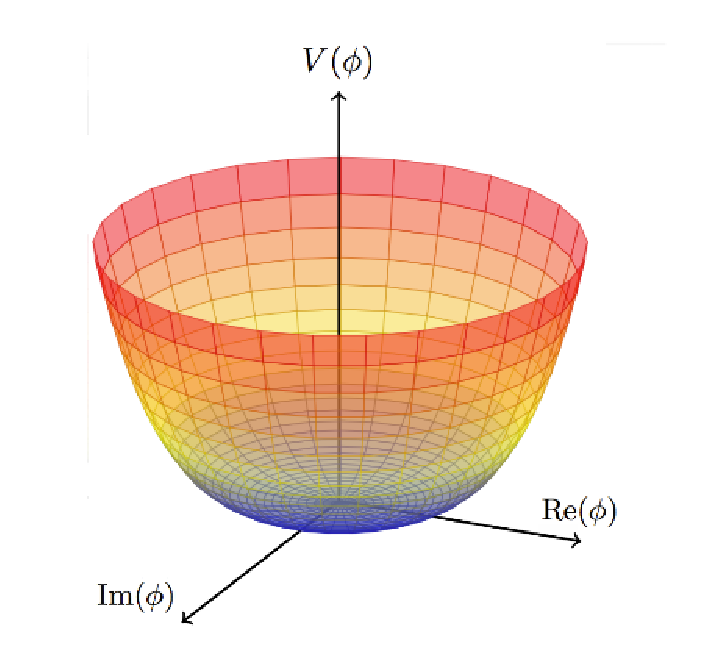
\includegraphics[width=0.45\textwidth]{theory/figures/higgs1.eps}}
	\subfigure[]{\label{fig:higgs2}
  	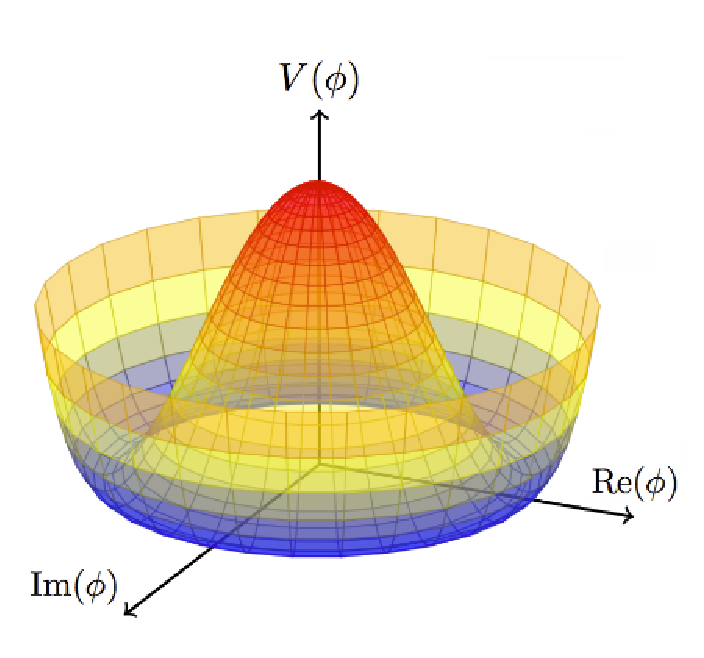
\includegraphics[width=0.45\textwidth]{theory/figures/higgs2.eps}}
	\caption{Vacuum pontential for $\lambda>0$ and (a) $\mu^2>0$ or
          (b) $\mu^2<0$, with the typical shape of a mexican hat~\cite{Michael:1569839}.}
\end{center}\end{figure}

\begin{equation}\label{eq:vacuum}
\phi_{0} = \begin{pmatrix} 0 \\ v/\sqrt{2}
\end{pmatrix}
\end{equation}
where $v = \sqrt{-\mu^{2}/\lambda}$ is 
the vacuum expectation value. Finally, since
only the vector bosons got their mass up to now
by directly ``eating'' the Goldston bosons
(while the fact that $U(1)_{Q}$ is unbroken 
causes the photon to remain massless),
the only thing left to do is to introduce 
the scalar-fermion interaction in order to give
mass to the fermions. This is done defining
an explicit Yukawa coupling $G_{lept}$ that gives:
\begin{equation}\label{eq:lagYukawa}
\mathcal{L}_{Yukawa} = -G_{lept}\big[\bar\psi_{R}(\phi^{\dag}\psi_{L}) + (\bar\psi_{L}\phi)\psi_{R}\big] .
\end{equation}Thus the complete electroweak Lagrangian of the SM, that can be generalized also to quarks (see Table \ref{tab:isospin}), is\begin{equation}\label{eq:lagSM}
\mathcal{L}= \mathcal{L}_{lept} +\mathcal{L}_{gauge} +\mathcal{L}_{\phi} +\mathcal{L}_{Yukawa}.
\end{equation}

\begin{table}[htb]\centering\begin{tabular}{cccc}\toprule
\multicolumn{4}{c}{Weak isospin left-handed doublets \bfseries $\psi_{L}$} \\ \midrule \\ 
$\begin{pmatrix} \nu_{e_{L}} \\ e_{L} \end{pmatrix}$ & $\begin{pmatrix} \nu_{\mu_{L}} \\ \mu_{L} \end{pmatrix}$ &$\begin{pmatrix} \nu_{\tau_{L}} \\ \tau_{L} \end{pmatrix}$ & \bfseries Leptons \\ \\ 
$\begin{pmatrix} u_{L} \\ d'_{L} \end{pmatrix}$ & $\begin{pmatrix} c_{L} \\ s'_{L} \end{pmatrix}$ &$\begin{pmatrix} t_{L} \\ b'_{L} \end{pmatrix}$ & \bfseries Quarks \\
 \\ \bottomrule\\ \toprule
\multicolumn{4}{c}{Weak isospin right-handed singlets \bfseries $\psi_{R}$} \\ \midrule \\ 
$ e_{R} $ & $ \mu_{R}$ &$\tau_{R}$ & \bfseries Leptons \\ \\ 
$u_{R}$ , $d'_{R} $ & $c_{R}$ , $s'_{R} $ &$ t_{R}$ , $b'_{R}$ & \bfseries Quarks \\
 \\ \bottomrule
\end{tabular}\caption{Weak isospin multiplets. $q'$ refers to the flavour eigenstate that correspond to the mass eigenstate transformed with the CKM matrix.}\label{tab:isospin} \end{table}

An important consequence of the introduction of the scalar Higgs 
field and the consequent spontaneous symmetry breaking
is the mixing of the vector bosons $B_{\mu}$ and $W^{1,2,3}_{\mu}$ 
to give the photon $A_{\mu}$, the two $W^{\pm}_{\mu}$ and 
the $Z_{\mu}$ bosons:
%\begin{equation}\label{eq:AZ}
%\left \{ \begin{array}{ll}
%A^{\mu} = \cos\theta_{W}B^{\mu} + \sin\theta_{W}W_{3}^{\mu}\\
%Z^{\mu} = -\sin\theta_{W}B^{\mu} + \cos\theta_{W}W_{3}^{\mu}\end{array}\right. ,
%\end{equation}
\begin{align}
  W_{\mu}^{\pm} & = \frac{1}{\sqrt{2}}\left(W_{\mu}^{1}\mp i W_{\mu}^{2}\right), \label{eq:Wpm} \\
  \left(
  \begin{array}{c}
  A_{\mu} \\ Z_{\mu}
  \end{array}
  \right)
  & =
  \left(
  \begin{array}{cc}
  \cos\theta_{W} & \sin\theta_{W} \\
  -\sin\theta_{W} & \cos\theta_{W}
  \end{array}
  \right)
  \left(
  \begin{array}{c}
  B_{\mu} \\ W_{\mu}^{3}
  \end{array}
  \right) , \label{eq:AZ}
\end{align}
where the Weinberg angle $\theta_{W}$ is defined through\begin{equation}\label{eq:weinb}
\left \{ \begin{array}{ll}
\dfrac{g}{\sqrt{(g')^{2}+g^{2}}} = \cos\theta_{W} \\
\dfrac{g'}{\sqrt{(g')^{2}+g^{2}}} = \sin\theta_{W} \end{array}\right. .
\end{equation} 
The mass terms that arise from the Higgs mechanisms are finally:
\begin{align}
  m_W & =  \dfrac{1}{2}vg \quad \quad \quad & \textnormal{for} & \quad \quad \quad
  & W^{\pm}_{\mu} & = \dfrac{1}{\sqrt{2}}\left(W^{1}_{\mu} \mp i W^{2}_{\mu}\right), \quad & \\
  m_Z & =  \dfrac{1}{2}v\sqrt{g^{2}+{g'}^{2}}
  \quad \quad \quad & \textnormal{for} & \quad \quad \quad
  & Z_{\mu} & = \dfrac{gW^{3}_{\mu} - g'B_{\mu}}{\sqrt{g^{2}+{g'}^{2}}}, \quad & \\
  m_{\gamma} & =  0
  \quad \quad \quad & \textnormal{for} & \quad \quad \quad
  & A_{\mu} & = \dfrac{g'W^{3}_{\mu} + gB_{\mu}}{\sqrt{g^{2}+{g'}^{2}}}, \quad & 
\end{align}
$m_l = v G_{lept}/\sqrt{2}$ for leptons and $m_H = v\sqrt{2\lambda}$ for the Higgs boson. 
The experimental values for the masses of Standard Model particles
are listed in Table \ref{tab:mass}.


\begin{table}[htb]\centering

%\begin{minipage}{.2\textwidth}
    \begin{tabular}{cccc}\toprule
      Spin-$1$ & \multirow{2}{*}{mass} & Spin-0 & \multirow{2}{*}{mass}\\
      gauge bosons & & scalar boson & \\\midrule
    $\gamma$      & 0  & \multirow{4}{*}{$H$} & \multirow{4}{*}{$\sim 125~\gev$}                        \\
    $g$           & 0  & &                        \\
    $W^{\pm}$ & $ 80.385 \pm 0.015 \gev$ & &\\
    $Z$       & $ 91.188 \pm 0.002 \gev$ & &\\\bottomrule
    \end{tabular}

%\end{minipage}\begin{minipage}{.7\textwidth}
    \begin{tabular}{ccccccc}\toprule
      Spin-$\tfrac{1}{2}$ &  \multicolumn{2}{c}{\multirow{2}{*}{I generation}}
      &  \multicolumn{2}{c}{\multirow{2}{*}{II generation}}
      &  \multicolumn{2}{c}{\multirow{2}{*}{III generation}}\\
      fermions & & & & & \\\midrule
    \multirow{2}{*}{leptons} &
    $\nu_{e}$   & \small{$\sim 0$} &  
    $\nu_{\mu}$ & \small{$\sim 0$} &  
    $\nu_{\tau}$ & \small{$\sim 0$} \\
    &
    e            & \small{$511\kev$}   &  
    $\mu$ & \small{$105.7\mev$} &  
    $\tau$     & \small{$1.777\gev$} \\
    \multirow{2}{*}{quarks} &
    u & \small{$1.7-3.1\mev$}         &  
    c & \small{$1.29^{+0.05}_{-0.11}\gev$}  &  
    t & \small{$173.2^{+0.87}_{-0.87}\gev$}\\ %$172.9^{+1.1}_{-1.1}\gev$} \\
    &
    d & \small{$4.1-5.7\mev$} &  
    s & \small{$100^{+30}_{-20}\mev$} &  
    b & \small{$4.19^{+0.18}_{-0.06}\gev$} \\\bottomrule
    \end{tabular}
%\end{minipage}
  \caption{Experimental values for the elementary particles of the Standard Model.\label{tab:mass}}

\end{table}


\subsection{Adding the strong interaction}\label{sec:qcdlagr}

Adding the color transformations $SU(3)_{C}$, the Standard Model is
finally described by the symmetry group 
$SU(3)_{C}\otimes SU(2)_{L}\otimes U(1)_{Y}$.
In the same way electromagnetic interactions are 
described by Quantum ElectroDynamics (QED), 
strong interactions are described by Quantum ChromoDynamics (QCD~\cite{Ecker}).
However, while the photon does not carry electric charge,
the gluon does carry color charge (in particular it exists in
eight states, being a color octet) and can, therefore, self-interact.

The QCD lagrangian only involves quarks and gluons, and reads:
\begin{equation}
\left \{ \begin{array}{cl}
\mathcal{L}_{QCD} &=\;\; \sum\limits_{f=1}^{6}\bar{q}(i\gamma^\mu D_\mu - m_q)q 
                    -\frac{1}{4}F^{\mu\nu}_{a}F^{a}_{\mu\nu}\\
 D_\mu &=\;\; \partial_\mu + ig_sG_\mu^a T^a\\
  F^{a}_{\mu\nu} &=\;\;  \partial_\mu G_\nu^a - \partial_\nu G_\mu^a - 
                    g_sf^{a}_{\ bc}G^b_\mu G^c_\nu
\end{array} \right.
\end{equation}
where $q$ is the quark field and $m_q$ is the quark mass, summed over 
the six flavors ($f$) of quarks, and $a$ runs over the eight degrees of 
freedom of the gluon field, $T^a$ being the generators
of the $SU(3)_C$ group. The field tensor $F^{a}_{\mu\nu}$ 
is derived from the gluon field $G_\mu^a$ and 
its third term describes the gluon self-interaction, with
$f^a_{\ bc}$ being the structure constants
of the $SU(3)_{C}$ group. 
%non-abelian nature  of the QCD, and it describes the
The strong coupling constant $\alpha_s$ is defined
as  $\alpha_s=g_s/4\pi$ and its values, large at
low energies (i.e. large distances), and small at high 
energies (i.e. short distances), determine the 
peculiar property called {\it asymptotic freedom} which
explains the confinement of the quarks inside the hadrons
(see Figure~\ref{fig:alpha_s}). Indeed, at
small distances $\alpha_s$ is so small that
the strong interaction can be treated perturbatively
and quarks and gluons described as free particles.
On the other hand, a quark cannot be found
isolated since at large distances the field strength
will increase enough to create new quarks 
from the vacuum and colorless hadrons will be formed.

\begin{figure}[tbph]
\begin{center}
\subfigure{
  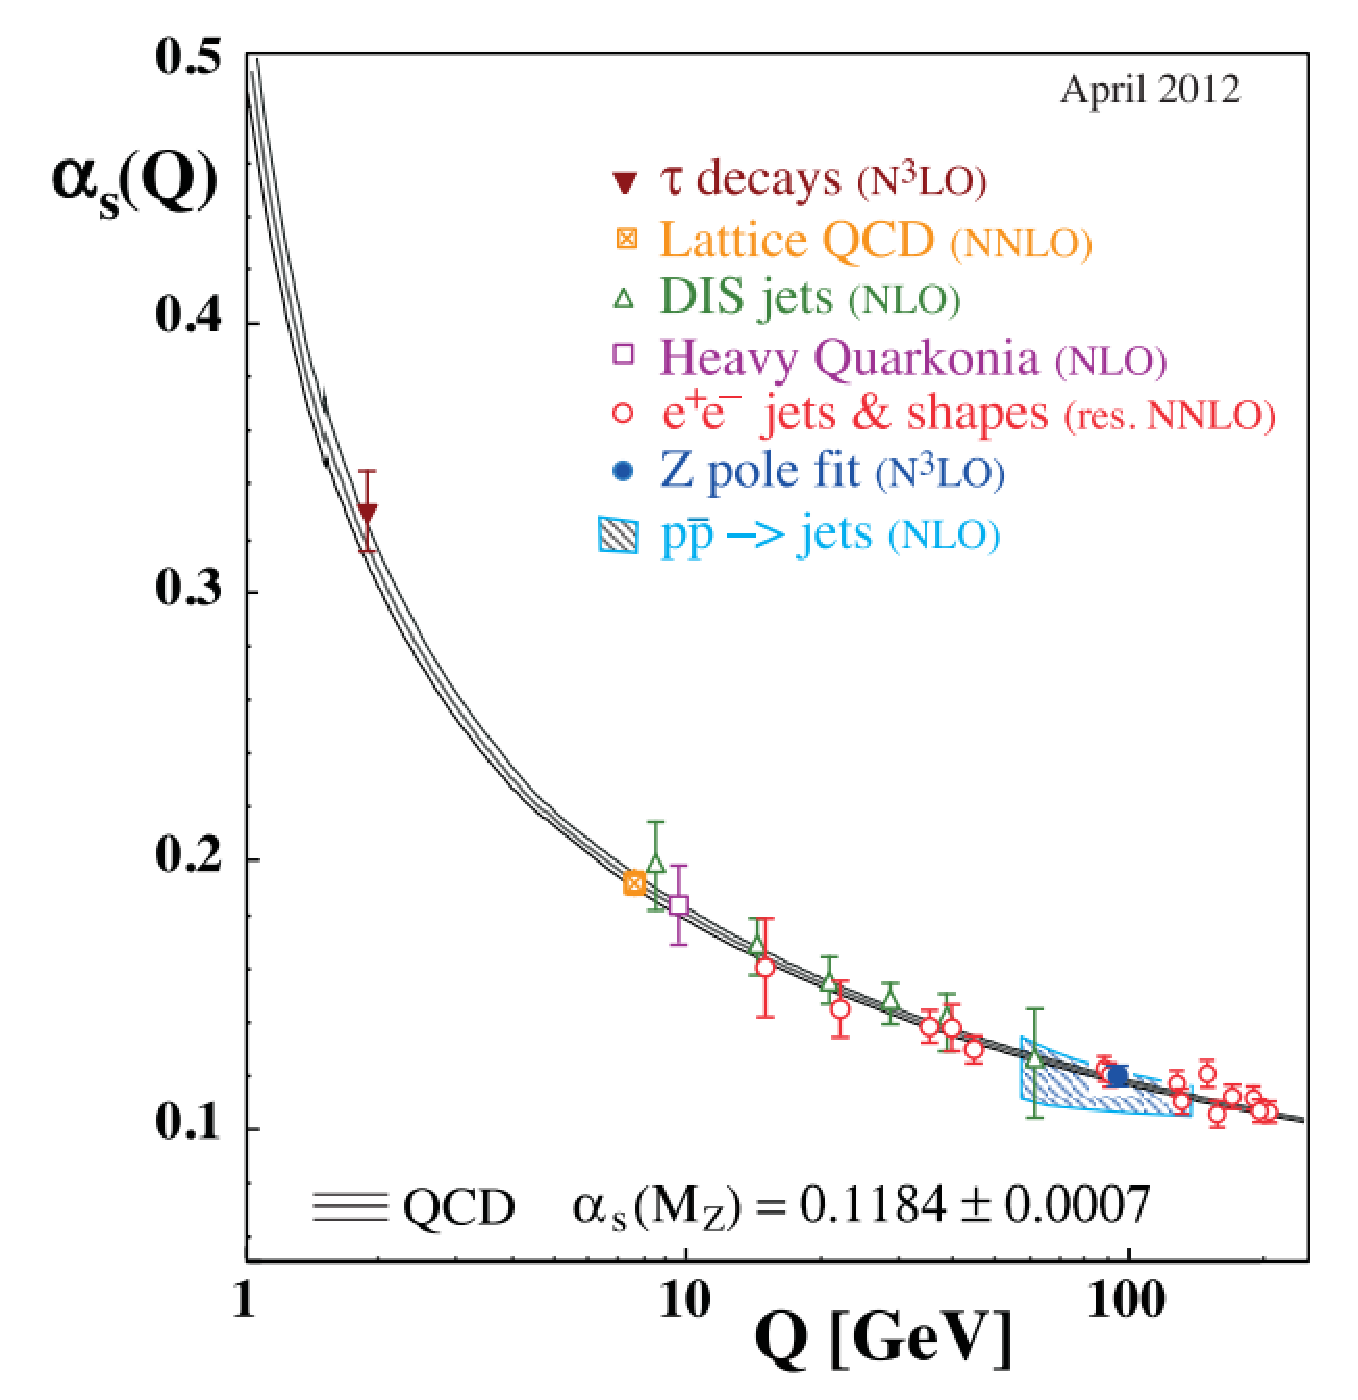
\includegraphics[width=0.5\textwidth]{theory/figures/asq-2012.eps}
}
\caption{Running of the strong coupling $\alpha_s$ with the energy scale $Q$,
proven from different measurements~\cite{alpha_s}.}
\label{fig:alpha_s}
\end{center}
\end{figure}

As an example of how quarks behave in hadrons,
protons are composed of two {\it valence} up quarks
and one {\it valence} down quark. The quarks continuosly
exchange gluons, which create in turn quark-antiquark pairs,
resulting in what is referred to as a ``sea'' 
of quarks and gluons. 
%randomly created and annihilated in vacuum fluctuations. 
As the sum of the rest masses of the valence quarks contributes 
only to about 1\% of the total nucleon
mass, what accounts for the missing 99\% is the
binding energy of gluons and sea quarks.
Further details on QCD will be given in Section~\ref{sec:MCphenomenology},
where the phenomenology of proton-proton collision
is discussed.



\subsection{Experimental success of the Standard Model}\label{sec:THsuccess}

Even if the SM was somehow born to be merely a stepping stone, 
it consolidated through the years, standing all experimental tests 
sometimes with a precision greater than 0.1\%. Experiments carried 
out at the Large Electron-Positron (LEP) collider at CERN, 
thanks to the clean signals given by $e^{+}e^{-}$ collision events, 
allowed to obtain very high precision measurements of the SM parameters
(see Figure~\ref{fig:smparam}). %for a summary of the measurements, with their errors, of the free parameters of the SM).
\begin{figure}[htb]\begin{center}
	\subfigure[]{\label{fig:smparam}
  	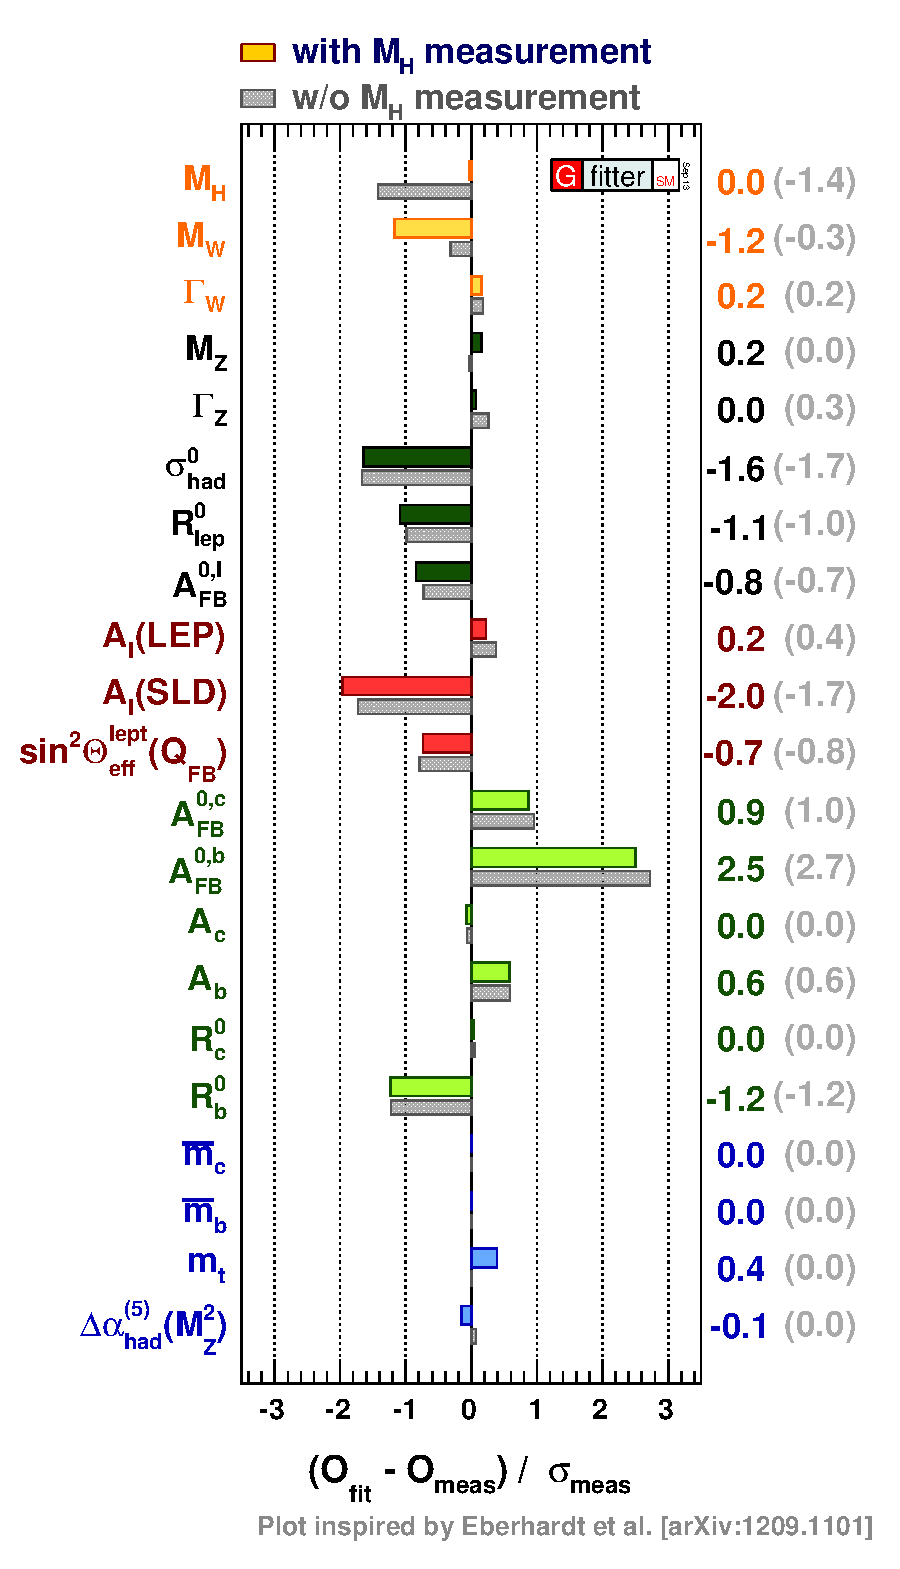
\includegraphics[width=0.35\textwidth]{theory/figures/fitSM_new.eps}}%cernlep5_5-04}}	
	\subfigure[]{\label{fig:WtopMass}
  	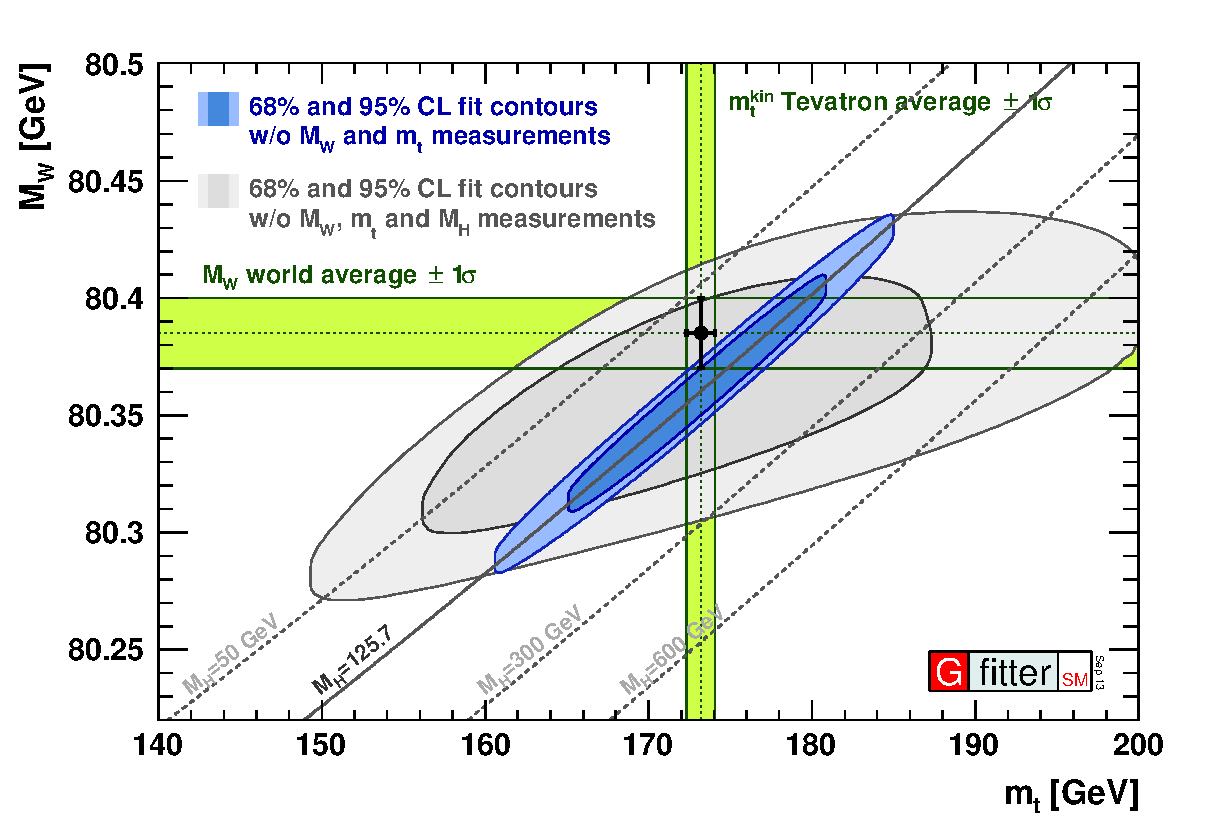
\includegraphics[width=0.6\textwidth]{theory/figures/W_vs_top.eps}}
        \caption[bla]{(a) Comparing fit results with direct measurements
of the free parameters of the SM, with the fit performed
with and without inclusion of the measured $M_H$. 
The pull values are defined as deviations between experimental 
measurements and theoretical calculations in units of the experimental uncertainty~\cite{Baak:2012kk}. 

        (b) Contours of 68\% and 95\% confidence level obtained 
from scans of fits with fixed variable pairs 
$M_W$ vs. $m_t$. The narrower blue and larger 
grey allowed regions are the results of the 
fit including and excluding the $M_H$ measurements, 
respectively. The horizontal bands indicate the 1$\sigma$
regions of the $M_W$ and $m_t$ measurements (world averages)~\cite{Baak:2012kk}. 
}
%Measured free parameters of the SM with the corresponding
%precision and the result of the consistency fit~\cite{Renton}.\label{fig:smparam}}
%\url{http://cerncourier.com/cws/article/cern/29076}}
\end{center}\end{figure}
 
In particular, the LEP experiments (ALEPH, DELPHI, L3 and OPAL) performed the measurements 
of the $Z$ boson mass with a precision of 0.0023\%, that made it one of the most 
precisely known quantities within the SM. %AAAAAAAAAAAAAAAAA \footnote{Note that the masses of the $W$ and $Z$ bosons are not predicted by the theory, but their ratio is (see Section~\ref{sec:ewlagr}).}. 
Furthermore, measurements of its total 
decay width and of its partial decay widths for all processes with a 
visible final state (i.e. different from $\nu\bar\nu$) allowed to set 
the number of light neutrino flavours to three, confirming the three-generation 
SM and excluding the possibility for a fourth family of leptons with masses
 lower than half of $m_Z$.

The penultimate discovery inside the SM has been the observation of the 
top quark in 1995 at the Fermilab's experiments CDF and 
D0~\cite{PhysRevLett.74.2626,PhysRevLett.74.2422}. 
The mass of the top quark resulted consistent with the predicted 
constraints (see Figure~\ref{fig:WtopMass}), 
thus confirming again the SM as an accurate framework. 
Figure~\ref{fig:history_mt} shows the evolution in
time of the top quark mass measurements and predictions,
while in Figure~\ref{fig:comb_mt} the best average
from measurements performed at the Tevatron experiments
CDF and D0 is given. All the properties that have been
observed (see for a review e.g.~\cite{Wicke:2010cg})
proved the top quark to be the SM up-type quark of the third generation.
At that point, and for almost 20 years, the last missing piece whose
absence could invalidate all the previous beautiful corroborations, was
the observation of a Higgs boson with a light mass for  self-consistency 
of the overall fit of data. When the LEP physics program was terminated,
direct searches gave, at 95\% CL, a lower limit of 114~\gev\ and an upper 
limit of 144~\gev\ on the mass of the Higgs boson~\cite{Barate:2003sz}. %,Renton}.

\begin{figure}[hbtp]
\begin{center}
	\subfigure[]{\label{fig:history_mt}
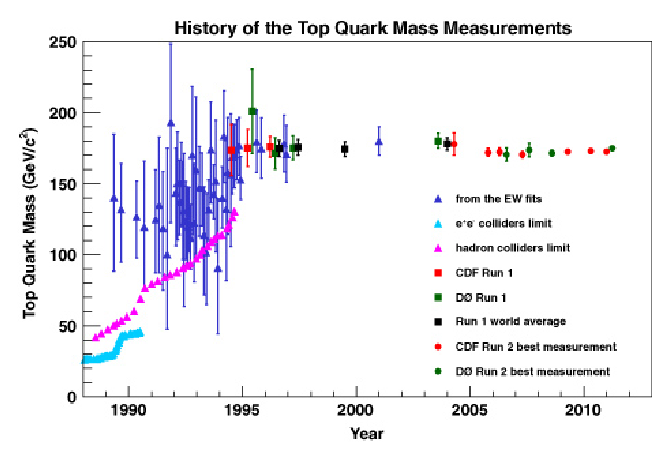
\includegraphics[width=0.6\textwidth]{theory/figures/rpp347183f01_online}}
%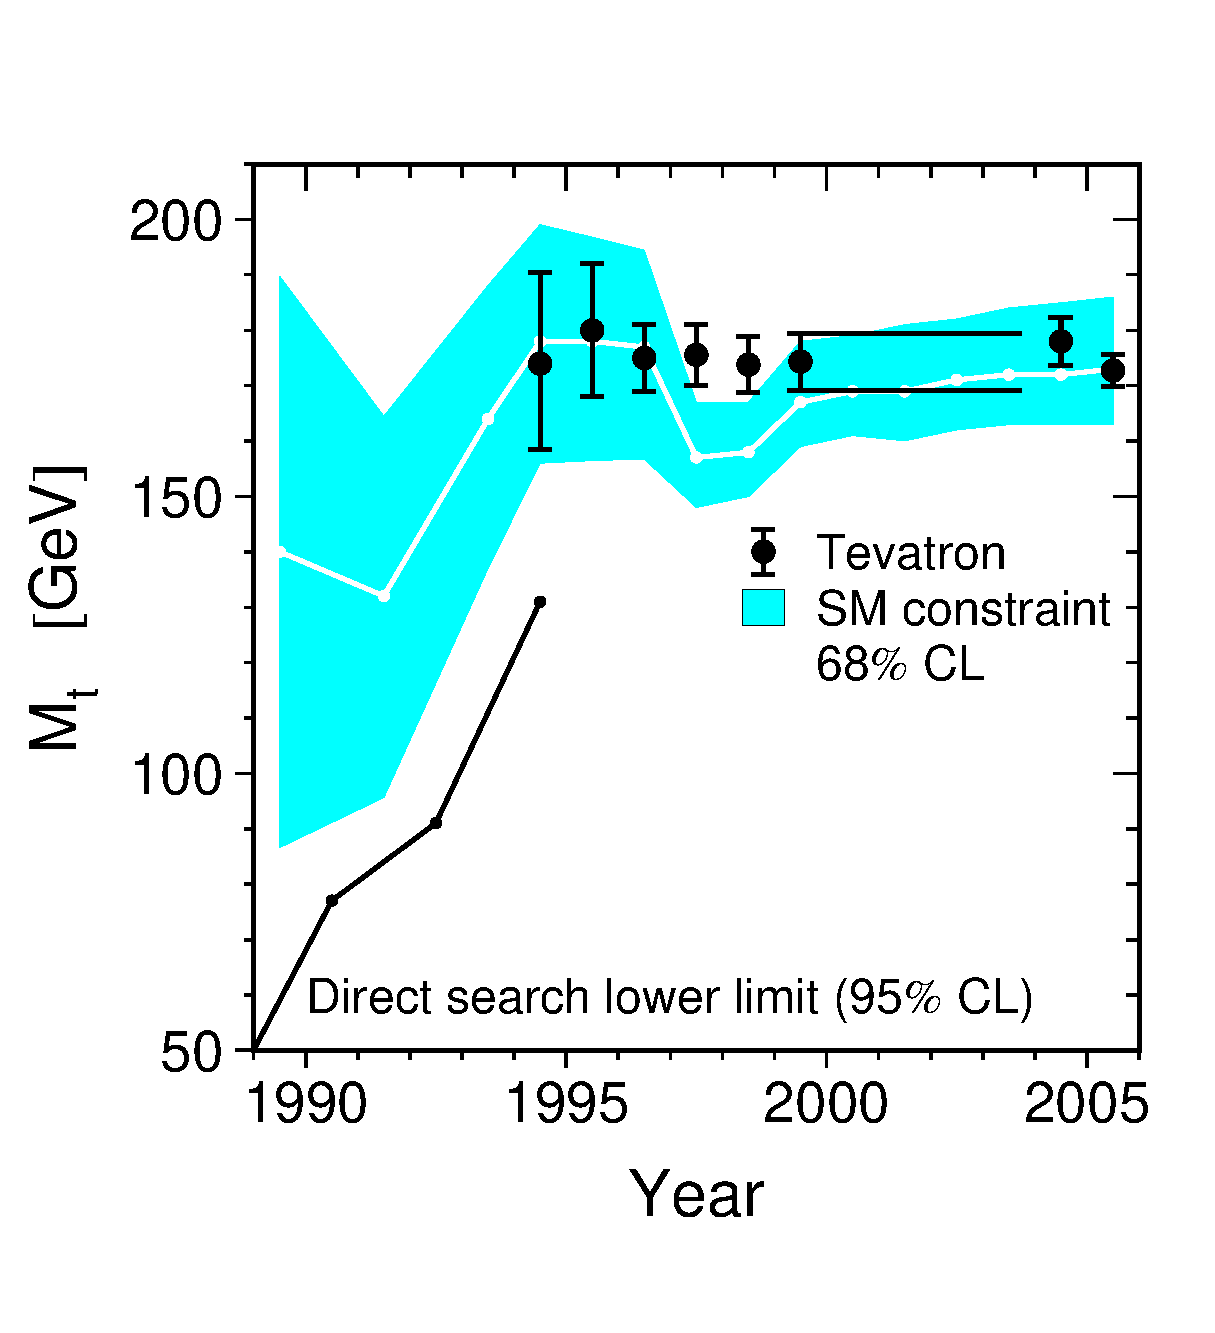
\includegraphics[width=0.5\textwidth]{theory/figures/history_mt}}
	\subfigure[]{\label{fig:comb_mt}
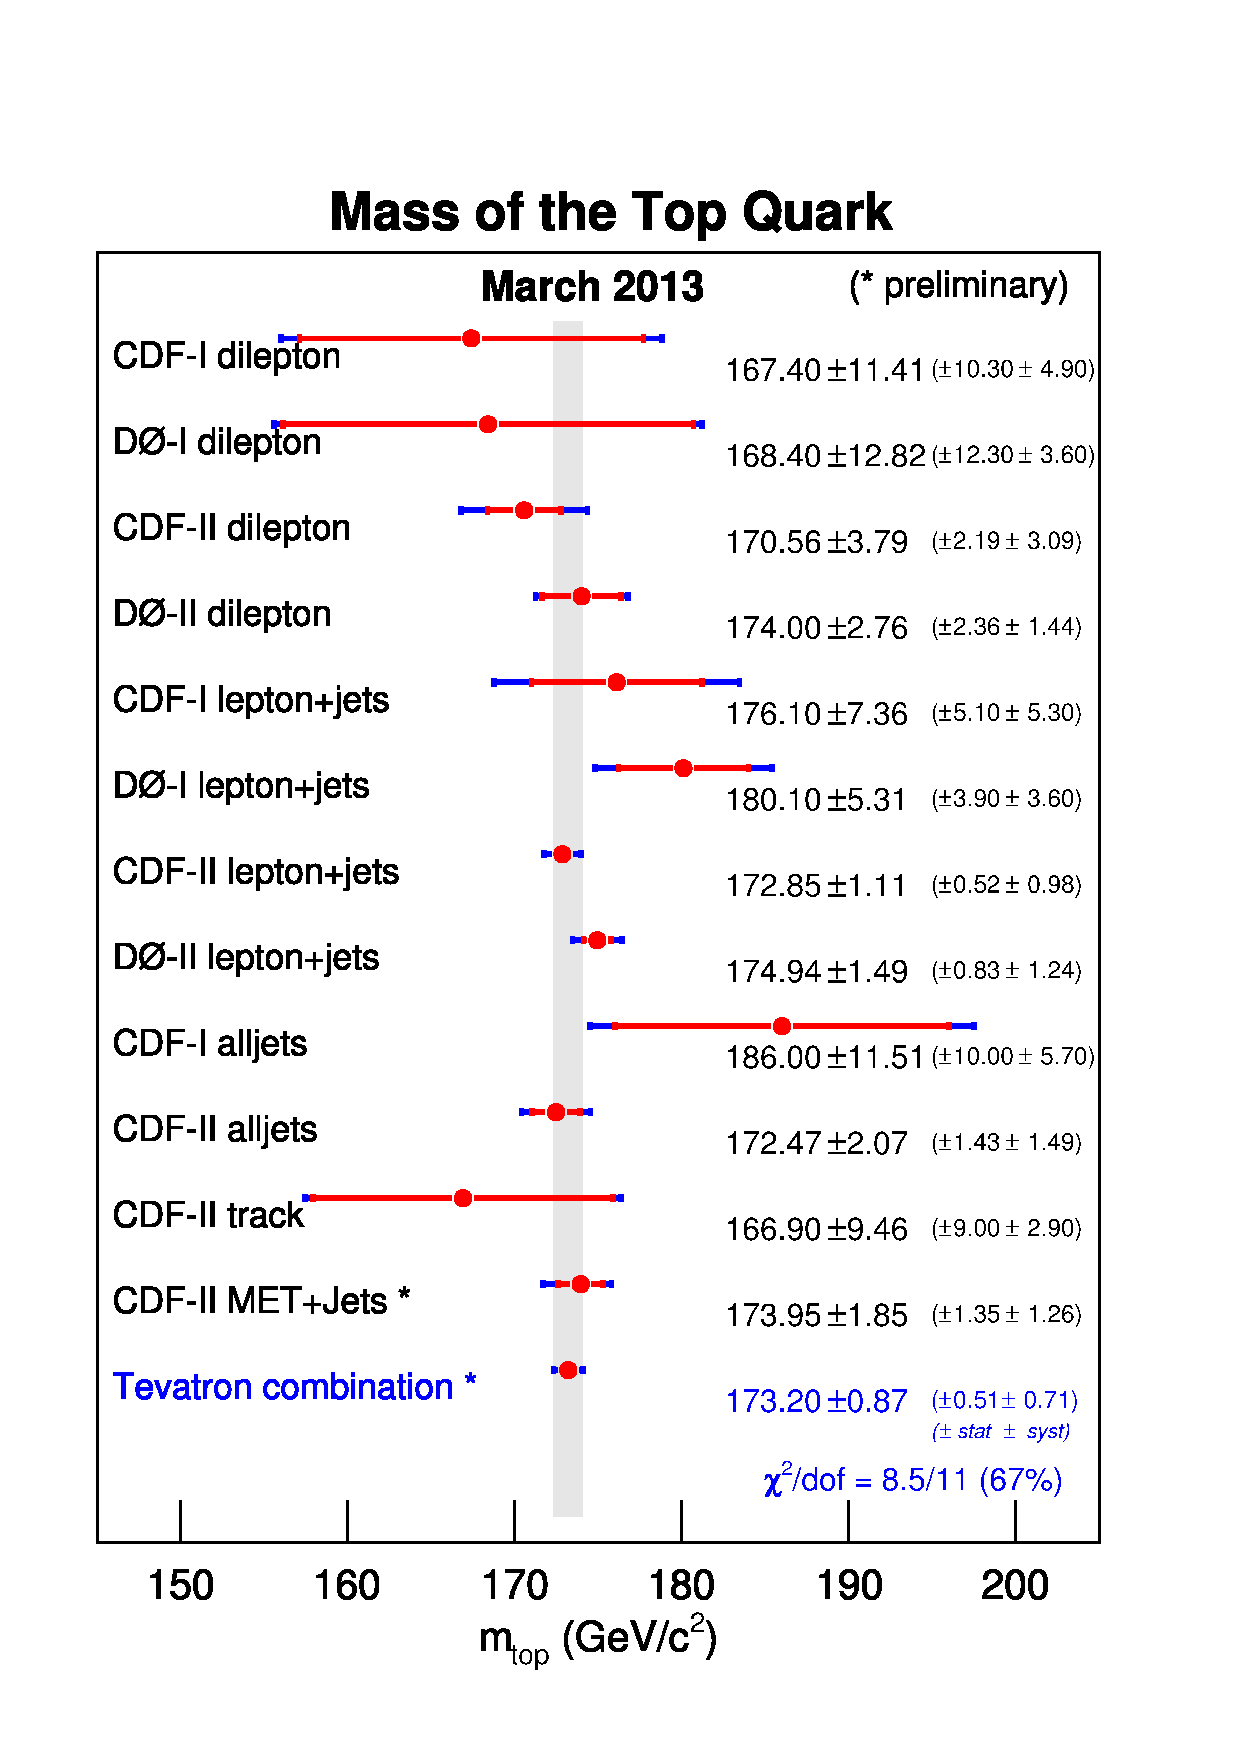
\includegraphics[width=0.35\textwidth]{theory/figures/TevMtWin13-2digit}}
\caption{(a) Evolution in time of the top mass prediction from
EW fits, of its exclusion limits at colliders and of its
experimental measurements at Tevatron~\cite{Galtieri:2011yd}.
(b) Summary of the top mass measurements at the CDF and D0 experiments
from Run-I (1992-1996) and Run-II (2001-present) 
in various channels and the resulting Tevatron average
 mass of the top quark~\cite{CDF:2013jga}.}
\end{center}
\end{figure}




Then LEP was dismantled, the LHC was built, and in 2012 
the ATLAS and CMS experiments
observed a new $\sim$125~\gev\ mass boson~\cite{2012gk,Chatrchyan201230}
with the same spin-parity as the one expected from a Standard Model
Higgs boson~\cite{Aad:2013xqa,CMShiggsspin}. 
A precise identification of this new particles, necessary
in order to say the final word about its nature (is it a Higgs boson?
Is it the Standard Model Higgs boson? Is it a ``new physics'' Higgs boson?),
is expected to come within the next decades of activity of the LHC and its
experiments. Up to the time of the writing of this dissertation, the most
recent results from the ATLAS and CMS experiments measuring the
properties of the new particle show consistency with a Standard
Model Higgs boson~\cite{Aad:2013wqa,CMS-PAS-HIG-13-005}.




\section{Unanswered questions and new physics quests}\label{sec:THquest}

In the case the new boson discovered in July 2012 
really is a Standard Model Higgs boson, there would
be no more arguments to contradict the Standard Model
as an {\it effective theory}. Indeed many facts, both 
in theory and experiments, hints that the Standard Model,
despite is great success in describing the interaction
of fundamental particles, might be just an approximation
at low energy regimes of a more complete theory.

One of the principal objections to the Standard Model as 
``the final theory'' is the high number of arbitrary parameters 
of the theory. In fact, 19 parameters are needed to fit 
data from experimental observations. 
Three of them  are the couplings of the gauge groups 
$g_3, g, g'$ for the strong, electromagnetica and weak 
interactions respectively, also written as: 
\begin{equation}\label{eq:couplings}
\alpha_{s}=\dfrac{g_{3}^{2}}{4\pi} ,\quad 
\alpha_{elm} = \dfrac{e^{2}}{4\pi} =  \dfrac{g^{2}\sin^{2}\theta_{W}}{4\pi}, 
\quad \sin^{2}\theta_{W} = \dfrac{(g')^{2}}{g^{2}+(g')^{2}}.
\end{equation}
Then, 13 parameters are associated with the nine charged 
fermion masses and the four parameters of the CKM matrix 
(three quark-mixing angles and one phase), 
two are needed to describe the Spontaneous Symmetry Breaking mechanism, 
i.e. the Higgs vacuum expectation value $v$ and 
the quartic coupling constant $\lambda$, and the last one is the 
QCD $\theta$ parameter. Additionally, if neutrinos are massive 
(as it is almost certain from neutrino oscillation observations, 
see e.g. \cite{Langacker:817840}) there will be even more arbitrary 
parameters describing their masses and their mixing. 
Furthermore, massive neutrinos cannot exist in the Standard
Model, where only left-handed neutrinos are predicted and thus
no Dirac mass term can appear\footnote{A way out of this
problem postulates a new type of neutrinos, namely 
{\it Majorana neutrinos}, in contrast to {\it Dirac neutrinos}.}.


%If, based on these considerations,  one assumes that 
The arbitrariety of parameters, and in particular of the
fermion masses, introduces what goes under the name of
{\it naturalness problem}. A ``natural'' theory is
characterized by free parameters with values at, more or
less, the same order of magnitude. This does not happen in
the Standard Model, where the top quark, as an example,
has a mass $\sim 10^5$ larger than the up quark.
This issue further develops as follows. If the 
Standard Model is valid only up to  an energy scale 
$\Lambda$ (which, if it's the Planck scale, differs
from the electroweak scale by $\sim 10^{17}$!), 
then the scalar Higgs boson mass 
should encounter radiative corrections from 
vacuum polarization diagrams (like the one in Figure~\ref{topLoop}) 
of the order of $\Lambda$ giving to the mass the 
value: %~\cite{dawson-1997}:
\begin{equation}\label{eq:higgsMass}
M_{H}^{2} \sim M_{H_{0}}^{2} 
+ \dfrac{\lambda}{4\pi^{2}} \Lambda^{2} 
+ \delta M_{H}^{2}. \end{equation}
If the mass counterterm $\delta M_{H}^{2}$ does not 
cancel the quadratically divergent contribution and 
if the cutoff scale is chosen as the Planck scale, then
\begin{equation}
M_{H}^{2} \sim 10^{32},\end{equation} 
i.e. many orders of magnitude bigger than the experimentally 
measured value coherent with the Standard Model 
and with the unitarity constraint. This  
is the \textit{hierarchy problem}, and 
could be fixed within the Standard Model by 
choosing a fine-tuned mass counterterm, a 
solution considered not really elegant also 
because fine tuning will be required for every 
order in the perturbative expansion\footnote{This 
problem does not arise with loop corrections to 
fermion masses, which are protected by chiral 
symmetry, nor with boson masses,
which are protected by gauge invariance. It
is, actually, an issue of scalar particles
like the Higgs boson.}. %and that's the reason why fermion masses are said to be ``natural''.} 


\begin{figure}[htb]\begin{center}
%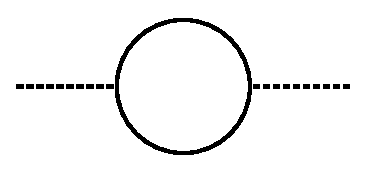
\includegraphics[width=.2\textwidth]{theory/figures/loop1}
\subfigure{ \def\svgwidth{0.25\textwidth}
\input{theory/figures/mod_loop1.eps_tex}}
\caption{The typical vacuum polarization diagram 
  for the Higgs is a top quark loop.}
\label{topLoop}\end{center}\end{figure}
%This argument looks the same of what made physicists pass from Fermi theory to Standard Model. In fact at that time the Fermi point like interactions were a good description of weak scattering processes of fermions $f+f\rightarrow f+f$, but the unitarity  predicted that at an energy $E_{crit} \sim 600$ GeV the theory would become inconsistent. Then it was found that new physics (the vector bosons of the Standard Model) was needed already from an energy scale about 100 GeV, maybe due to the small coupling constant of weak interaction. Now, the scattering process $W+W\rightarrow W+W$ has a scattering amplitude growing linearly to the self-coupling constant of the Higgs field $\lambda$. The formula for the critical energy is now related to the Higgs mass as \cite{Ho-Kim} $$\dfrac{E_{crit}}{v} = \exp\bigg(\dfrac{4\pi^{2}v^{2}}{3M_{H}^{2}}\bigg),$$ which for an higgs Higgs mass less than 150 GeV gives $E_{crit} \sim 10^{18}$, thus making the Higgs model valid up to that scale. However for an heavier Higgs with a mass about 700 GeV, such critical energy goes down to $10^{3}$ GeV.  It is to remark that in the electroweak interactions the Higgs contribution to radiative corrections is very low since is denoted by a logarithm function, thus giving low variations and not affecting the precision electroweak data. The meaning of this is, whatever the critical energy value will be, the Standard Model is an effective theory embedded in a more fundamental theory with $E_{crit}$ acting as a cutoff.

\begin{figure}[h!tb]\begin{center}
        \subfigure{ %\def\svgwidth{0.9\textwidth}
\input{theory/figures/mod_scales.eps_tex}}
	\caption{Typical length and energy scales
          of some of the fundamental parameters
          of the Universe.\label{fig:scales}}
\end{center}\end{figure}

Another disturbing feature of the Standard Model as it is 
is the lack of theoretical explanation for the generations 
of quarks and leptons to be exactly three, as suggested
(under certain assumptions) by precision measurements 
performed at LEP at the $Z$-pole ($\rts\sim 91$~\gev). 
From QCD comes the only constraint for quark generation
to be less that nine.

Cosmology and cosmological observations also challenge 
the Standard Model. The reason for baryon-antibaryon 
asymmetry is still not understood although we know 
that it is connected to  CP violation\footnote{The CP violating 
phase introduced in the CKM mechanism cannot, however, 
account for the total baryon-antibaryon asymmetry measured.}. 
Besides, astronomical observations~\cite{Ade:2013zuv} 
tell us that the energy density of the 
Universe is made only for a 4-5\% of ordinary baryonic 
matter, the other components being dark matter (20-25\%) 
and dark energy (70-76\%). Dark matter is non-baryonic 
matter that interacts only weakly and gravitationally and,
therefore, cannot be observed with telescopes but it
is revealed by its gravitational interaction with ordinary 
matter in space. 
It is now believed that Dark Matter is composed  of 
Weakly Interacting Massive Particles (WIMPs) whose 
masses range from a few GeV to a few TeV and  are 
not predicted within Standard Model. Dark energy instead is 
still more mysterious and maybe new physics will 
give some hints for its interpretation.

Another topic making the Standard Model likely to 
need improvements is the desire to go further in 
the unification of theories. Gravity is not 
implemented in the Standard Model, nor is available
a widely accepted quantum theory of gravity.
This is acceptable at the electroweak scale of 
few hundreds of GeV where the strength of gravity
is negligible, but its effect should become relevant 
going up to the Planck scale $\Lambda \sim 10^{19}$ GeV. 
Also, electroweak and strong forces forming the Standard 
Model gauge group $SU(2)_{L}\otimes U(1)_{Y}\otimes SU(3)_{C}$ 
are expected to unify at high energy since their coupling 
constants are running constants dependent on the energy 
scale (Figure~\ref{running}, $\alpha^{-1}_{i} = g^{2}_{i}/(4\pi)$). 
\begin{figure}[htb]\begin{center}
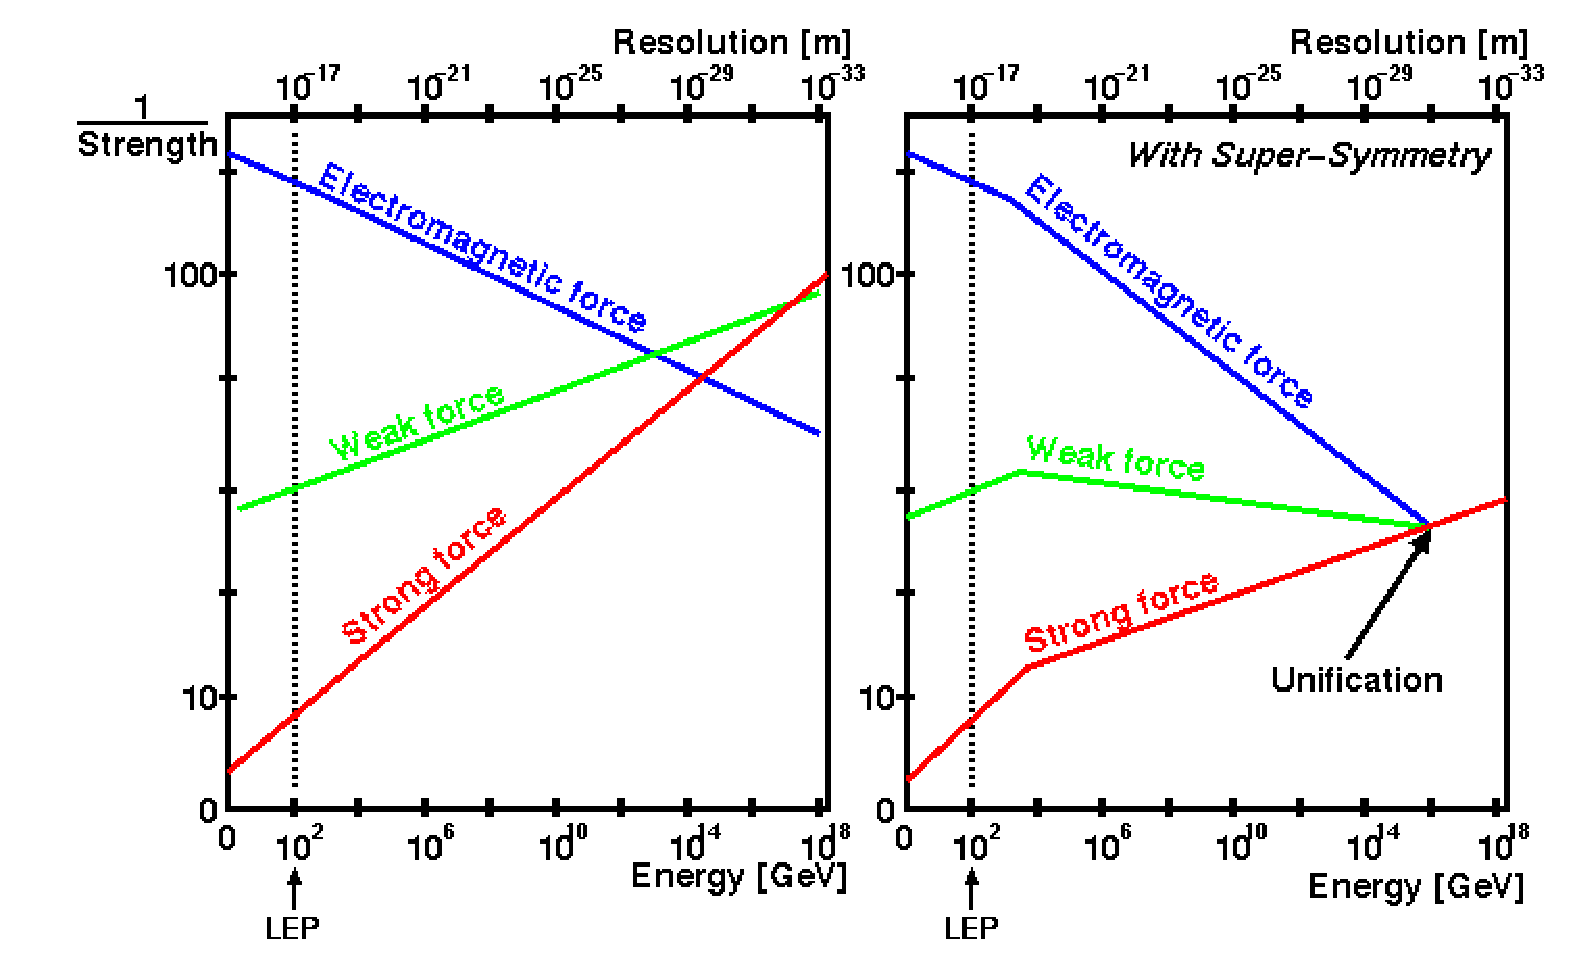
\includegraphics[width=.8\textwidth]{theory/figures/running_coupling}
\caption{Running coupling constants in the Standard Model (left) and 
in a hypothetical Supersymmetric Model (right, see Section~\ref{sec:susy}) 
as functions of the renormalization scale (picture from \url{http://scienceblogs.com},
original credits unknown). The energy scale explored at LEP is marked
on the two figures and corresponds to $10^2$~\gev. The LHC is able to
go just one order of magnitude further.}
\label{running}\end{center}\end{figure}

In the following some ``beyond-Standard Model'' (BSM) theories
proposed to solve most of the issues illustrated
before are briefly illustrated.

\subsection{Supersymmetry}\label{sec:susy}

Since Supersymmetry~\cite{Dawson:1996cq} is one of the most popular
BSM scenarios, having many trustful supporters even
now that after the first LHC run no trace of it
has been found, a brief explanation of its concepts
is included in this dissertation.

The basic idea is to postulate the invariance 
of the theory under a symmetry operation which 
trasforms fermionic fields into bosonic fields 
(and viceversa), called \textit{supersymmetry}. 
In this theory to each fermionic or bosonic 
degree of freedom of the Standard Model is associated a 
``superpartner''. These superpartners have all 
of the quantum numbers identical to the corresponding 
Standard Model particles, except for the spin quantum number 
transformed as $s' = |s - 1/2|$. Thanks to the 
presence of superpartners, the Fermi statistics 
allows to write the new version of Equation~\ref{eq:higgsMass} as:
\begin{equation}
\label{eq:higgsMassSUSY}
M_{H}^{2} \sim M_{H_{0}}^{2} + \dfrac{g_{F}^{2}}{4\pi^{2}} (\Lambda^{2} + m_{F}^{2} ) - \dfrac{g_{S}^{2}}{4\pi^{2}} (\Lambda^{2} + m_{S}^{2} ),
\end{equation} 
where the subscripts $F$ and $S$ indicate respectively 
fermionic and scalar degrees of freedom. If $g_{F} = g_{S}$ 
and masses are equal as in an unbroken supersymmetry scenario, 
the $\Lambda^2$ terms cancel and the hierarchy problem is solved. 
However, since no superpartners of known particles 
have been observed,  supersymmetry must be a broken 
symmetry and sparticles masses have to lie in an 
energy range not yet accessed by experiments.

%The simplest and most popular supersymmetric model is called the Minimal Supersymmetric extention of the Standard Model (MSSM). In the MSSM, $SU(2)_{L}\otimes U(1)_{Y}\otimes SU(3)_{C}$ gauge symmetries are still valid, but particles are now organized in \textit{Chiral Superfields} (formed by a complex scalar field and a fermion field with two components) and \textit{Vector Superfields} (made of a massless gauge field and two-component fermion field named \textit{gaugino}). Even if the scalar superpartners of fermions do not feature handedness, the chirality is formally assigned as the one of the standard particles in the supermultiplet. Then, for every family of quarks and leptons of the SM, a superfield made of an $SU(2)_{L}$ doublet of fermions and an $SU(2)_{L}$ doublet of scalars is defined ($\hat Q_{1,2,3}$ for quarks, $\hat L_{1,2,3}$ for leptons), as well as one superfield of right-handed anti-leptons and anti-sleptons ($\hat E_{1,2,3}$) and two superfields of right-handed anti-quarks and anti-squarks ($\hat U_{1,2,3}$ and $\hat D_{1,2,3}$). There are then two other Chiral Superfields in the Higgs sector ($\hat H_{u,d}$) and three Vector Superfields made of the gauge bosons and their relative superpartners ($\hat{G}^{a},\ \hat{W}^{i},\ \hat{B}$). 
%As can be seen in the summary of the MSSM supermultiplets in Table \ref{tab:supermultiplet}, an additional Higgs doublet needs to be postulated. The reason is that while in Equation \ref{eq:higgsMassSUSY} the term from scalar squarks cancels, in the similar equations for the fermions masses, where anomalies are automatically  cancelled within the SM, the newly introduced term from the Higgsino fermionic field remains. Thus another Higgs doublet with opposite $U(1)$ quantum number is defined. Furthermore, having two Higgs doublets is in general also required in order to give masses to both up and down type quarks in Supersymmetric theories. The two Higgs doublets with their eight components yield four extra bosons with respect to the SM, i.e. we get five physical Higgs bosons ($h^{0}, H^{0}, A^{0}, H^{\pm}$) and the relative superpartners, the fermionic Higgsinos. Gauginos mix  with Higgsinos resulting in the eight mass eigenstates: $\tilde{\chi}^{\pm}_{1,2}$ (the \textit{Charginos}) and $\tilde{\chi}^{0}_{1,2,3,4}$ (the \textit{Neutralinos}). After defining the superfields it is possible to construct the Lagrangian of the MSSM; a very clear step-by-step  pedagogical description for this task is given in Ref.~\cite{Martin}.

Supersymmetry also provides a natural candidate
for Dark Matter, the Lightest SUSY Particle (LSP), 
which, in a {\it R-parity}\footnote{The quantum number 
\textit{R-Parity} is defined as $R \equiv (-1)^{3(B-L) + 2s}$
to prevent lepton and baryon numbers from being violated.
It has value $+1$ for all Standard Model particles 
and $-1$ for their superpartners.} 
conserving scenario~\cite{Martin:1997ns},
would be stable, weakly interacting and neutral.



\subsection{Fourth generation SM4}\label{sec:sm4}

One of the simplest 


\subsection{Little Higgs}\label{sec:littlehiggs}

\begin{figure}[htb]\begin{center}
\subfigure{ \def\svgwidth{0.25\textwidth}
\input{theory/figures/mod_loop1.eps_tex}}
\subfigure{ \def\svgwidth{0.18\textwidth}
\input{theory/figures/mod_loop2.eps_tex}}
\label{fig:susyloops}\end{center}\end{figure}

\subsection{Extra-dimensions}\label{sec:extradimensions}





\section{Going beyond the SM with vector-like quarks}\label{sec:THvlq}

\cite{AguilarSaavedra:2009es,Martin:2009bg}

